\section{Background}

An important component of systems biology is the determination and
study of protein-protein interactions (PPIs) and the networks, or
interactomes, that they form. Previous work with single organism
systems has revealed PPI networks to be useful for annotating proteins
of unknown function \cite{karaoz2004whole,sharan2007network},
comparing organisms
\cite{kelley2003conserved,sharan2005conserved,dutkowski2007identification},
predicting other interaction types \cite{wong2004combining},
investigating the peptide regions guiding interactions
\cite{dinkel07,neduva06nuc,liu2010modular}, and identifying protein
complexes \cite{krogan2006global}. The study of single organism
networks has been extended to multiple organism host-pathogen
networks, where virus and cellular parasite proteins alter host
interaction networks by competing with host proteins for interactions
in the host network \cite{tournier06,sodhi04,dampier07}. As
experimental work with virus-host PPI networks has grown, the methods
for protein functional annotation and network comparison developed
using single organisms have been transferred to virus-host systems to
generate hypotheses about virus protein function \cite{calderwood07}
and investigate common viral strategies for countering the host immune
system \cite{navratil-system}.

\subsection{Virus-host network use cases}

The study of virus-host networks has not only aided antiviral drug
discovery and treatment optimization using existing drugs
\cite{brass08}, but furthered virology as well. Here we outline two
examples where the analysis of virus-host PPI networks yielded new
insights about viruses. The first case illustrates how virus-host
networks can be used to form hypotheses about the functions of
Epstein-Barr virus proteins. The second case describes a comparative
study of viral mechanisms for dealing with the host immune system that
was facilitated by knowledge of virus-host interactions.

Epstein-Barr virus (EBV), which has been linked to several diseases,
including cancer, is a herpesvirus that has almost 90 proteins
\cite{calderwood07}. 43 of these proteins are conserved across most
herpesviruses, and their functions have been investigated. However,
the functions of the remaining 46 proteins are not as well understood
\cite{calderwood07}. Determining functions these proteins was made
easier by generating and evaluating a virus-host network to help
formulate testable hypothesis about virus protein function
\cite{calderwood07}. Using the EBV-human PPI network, some EBV
proteins were hypothesized to have roles in cell survival and
apoptosis because the human proteins they interacted with were known
to have these functions \cite{calderwood07}. The possible involvement
of these EBV proteins in promoting cell survival and suppressing
apoptosis is important because these activities may be aiding the
progression of some cancers \cite{young2004epstein}. This transfer of
human protein function to virus proteins using virus-host PPI networks
has laid the ground work for future studies of virus proteins with
unknown functions.

Virus-host PPI networks have also been utilized to compare viral
strategies for subverting the human type I interferon response, which
consists of a four level cascade of interactions traveling from host
receptors, to adaptors and mediators, and ending at transcription
factors that initiate the immune response
\cite{navratil-system}. Navratil et al.\ constructed a human type I
interferon PPI network that included human proteins involved in the
type I interferon response, as well as human proteins that interacted
with these immune system proteins \cite{navratil-system}. Then the
interactions of proteins in this immune response network with virus
proteins from four viral families (Flaviviridae, Herpesviridae,
Papillomaviridae, and Retroviridae) were compared to find which of the
four levels of the type I interferon response were targeted
differently between viruses. All four virus groups were found to
preferentially interact with the signaling part of the immune
system. Viruses in the Flaviviridae and Herpesviridae families
targeted host proteins with many host interactions in the interferon
network, focusing on protein adaptors, mediators, and transcription
factors. Viruses in the Retroviridae and Papillomaviridae families
mostly targeted transcription factors. As more virus interactions with
host pathways are accumulated, this comparison of pathway specific
virus-host interactions can be extend to other host cellular
processes, such as apoptosis and autophagy.

% Gives us info about human evolution. What about pathways?

\subsection{Reasons for predicting virus-host interactions}

For studies of virus-host networks to continue, and to ensure that the
conclusions drawn from such networks are accurate, more interaction
data are needed. HIV has nearly fifteen hundred host proteins that
interact with its proteins \cite{fu09,ptak08}, but other viruses with
similarly sized proteomes, like hepatitis C virus (HCV), have less
than 500 virus-host interactions. This discrepancy in virus-host
interactome size is partially caused by the excessive study of
HIV-human interactions in comparison with other virus-host networks
\cite{mendez2010global}, but an additional contributor might be the
way in which virus-host interactions have been collected for HIV. With
the exception of HIV, virus-host interaction data have mostly been
generated by yeast two-hybrid screens. For instance, a recent study
investigating interactions between influenza and human proteins
identified less than 350 PPIs using a stringent two-hybrid assay that
required interactions to be present in primary and secondary screens
\cite{shapira2009physical}. Such stringency in screening is required
because of the significant false positive rates for high throughput
screens like yeast two-hybrid and tandem affinity purification assays
\cite{hart2006complete}. Stringent screens like the one used to
identify human-influenza virus interactions have low false discovery
rates, with estimates less than 15\% for yeast and worm protein
interactions \cite{huang2009precision}, but they often rule out many
true interactions, with false negative rates above 40\% for yeast and
worm \cite{huang2009precision}. False negative rates have been a
problem for yeast and human networks, yielding incomplete networks
that caused revisions of network properties and debates over
conclusions as networks grew in size \cite{batada06, batada07,
  agarwal09}. To make lasting conclusions from virus-host
interactions, we need nearly complete virus-host interactomes. Due to
the high false negative rates for high throughput screens, and based
on the multiple screens required to construct a high quality yeast PPI
network, several large-scale experiments will be required to
accurately map a virus-host network \cite{collins2007toward}, but
making predictions for virus-host interactions can aid in
accomplishing this goal by reducing cost and labor.

Experimental methods for determining protein interactions are costly
and require much time and effort, so methods to guide experiments or
replace them are desirable
\cite{skrabanek2008computational}. Predicted interactions for yeast
have helped to improve the accuracy, coverage, and efficiency of PPI
screens when used in combination with experiments
\cite{jansen2003bayesian,lee2004probabilistic}, and this will likely
translate to virus-host networks. There are two ways in which PPI
predictions can help in gathering additional virus-host
interactions. First, predictions can serve as an additional validation
of two-hybrid results. In recent high throughput influenza-human PPI
assays, interactions were required to pass two screens
\cite{shapira2009physical}. This approach to PPI investigation has
high false negative rates, but this could be solved by combining the
screens with predicted interactions. Instead of discarding all primary
screen interactions that failed to pass the secondary screen, only
those primary interactions with no prediction support would be thrown
out. These saved predicted interactions could then be tested in a
third screen. PPI predictions can also help to focus experiments that
are more thorough than two-hybrid screens, such as luciferase
complementation \cite{misawa2010rapid}. Computational approaches have
helped by reducing the number of host proteins to verify
experimentally \cite{lee2004probabilistic}. Predictions could be used
to find host pathways with which a virus interacts, and instead of
using the whole host proteome in assays, only host proteins appearing
in the prediction enriched pathways could be interrogated. In this
study, we describe a new method for how such predictions can be made
for virus-human interactions.

%% OK, so we should study them, but aren't the ones we have good enough?
%% Why is it important to predict interactions? What evidence is there
%% that the databases are incomplete? Let's look at the latest
%% virus-host interaction study, which concerned influenza
%% \cite{shapira2009physical}. For the virus-host protein interactions
%% for this study, Estimates of the coverage of single species two-hybrid
%% protein interaction maps. The known databases of virus-host
%% interactions are incomplete \cite{huang2007have,huang2009precision}.

%% Why is it important to predict pathways? Can't these be determined
%% from existing data?

\subsection{Predicting virus-host interactions} 

Previous host-pathogen interaction prediction methods focused largely
on finding PPIs between human and cellular parasite proteins. One
method found the probability that two protein domains interact given
the human PPI network, and used this probability to find the
likelihood that pathogen and human proteins interact given their
domain profiles \cite{dyer07}. Another method used structures of human
complexes as templates to match possible host-pathogen interactions
against, under the hypothesis that a candidate host-pathogen
interaction that resembles a host interaction is likely to represent a
real host-pathogen interaction \cite{davis07}. Candidate interactions
consisting of a pathogen and host protein were matched against
template host complexes using structural and sequence
similarity. Candidate interactions that were similar to a template
host complex were then subjected to a test that ensured that pathogen
and host protein were both expressed in the same tissue and at the
correct time in the pathogen's life-cycle. Translating these methods
to interactions between virus and human proteins has been difficult
because virus proteins have few domains and their structures are
either unsolved, or hard to find by comparative modeling. For
instance, to find structures for the N-terminal and C-terminal regions
of HIV VIF, two different protein structures were required for
comparative modeling \cite{lv07}. Due to problems with missing domains
and structures for virus proteins, in this chapter we address the
utility of an interaction prediction method that examines sequences
instead of structures, and utilizes small virus peptide motifs that
guide interactions instead of domains.

A study of HIV-human interactions conducted by Tastan et al.\ tried to
find the most predictive feature of virus-host interactions
\cite{tastan09}. In their method, each interacting virus-host protein
pair was associated with a feature vector composed of parameters
related to Gene Ontology (GO) \cite{ashburner00}, global gene
expression profiles, the human interaction network, human protein
domains, and HIV protein motifs. Using roughly one thousand direct
HIV-human interactions taken from the NCBI HIV-Human Protein
Interaction Database \cite{fu09,ptak08} as a training set, they
determined that the most predictive feature of virus-host interactions
was the number of host proteins with which the virus-host protein
pair's human protein interacted. The more interactions a human protein
had in the human interaction network, the more likely it was to
interact with a virus protein. While this is consistent with other
results from work with hepatitis C virus, Epstein-Barr virus, and
other human viruses that showed that virus targeted proteins had
significantly more host interactions that other proteins
\cite{calderwood07,dyer08,dechassey08}, it is not very useful for
comparative studies of virus-host interactions because it predicts
that all viruses interact with the same host proteins. For features
that differ between viruses, like virus peptide motifs that guide
protein interactions \cite{tonikian08,shelton08,kadaveru08}, Tastan et
al.\ estimated a relatively weak potential for predicting virus-host
interactions. Here we reevaluate this finding by using not only the
direct virus-host interactions evaluated by Tastan et al., but
indirect, regulatory interactions as well.

We focus this chapter on the computational identification of host
proteins targeted by an invading virus. We use HIV infection as a case
study because extensive study at the molecular level has yielded
nearly fifteen hundred HIV targeted human proteins, covering nearly
four thousand experimentally determined HIV-human interactions, which
are catalogued in the NCBI HIV-Human Protein Interaction Database. We
predict virus-host interactions based PPIs mediated by short
eukaryotic linear motifs (ELMs) \cite{puntervoll03} on HIV proteins
and human protein counter domains (CDs) known to interact with these
ELMs. It has been estimated that 15\% to 40\% of host protein
interactions are mediated by interactions involving a peptide motif
\cite{ceol2006domino,neduva2006peptides,petsalaki2008peptide}. The ELM
Resource has catalogued over 130 of these peptide motifs and
constructed a pattern that matches each one using documented motif
instances from the literature \cite{puntervoll03}. The ELM Resource
has also documented the protein CDs that interact with each motif. We
aim to obtain human protein sets enriched with sets of known virus
targeted proteins by annotating ELMs on HIV proteins, and using CDs on
human proteins to match them with HIV proteins based the ELM
Resource's catalogue of ELM and CD associations.

The potential functional roles of interactions mediated by ELMs and
their CDs in viral infection have been addressed in a number of recent
articles \cite{tonikian08,shelton08,kadaveru08}. The HIV literature
contains at least ten examples of HIV-human PPIs that are directly
associated with motif and domain presence. The motif/domain basis of
such PPIs is not restricted to a single HIV protein, but is widely
distributed across the HIV proteome, including HIV NEF \cite{roeth06},
ENV \cite{byland07}, TAT \cite{truant99}, REV \cite{truant99}, VIF
\cite{mehle06}, and VPU \cite{evrard06}. This experimental evidence is
the motivation for systematically investigating the association of
motif/domain pairs with PPIs between virus and host proteins. Although
Tastan et al. \cite{tastan09} estimated a relatively weak link between
binding motif presence and the actual virus-host PPIs, their work was
restricted to predicting direct binding between host and HIV
proteins. In this study, we set out to identify all virus-host
interactions, both direct and indirect, that have been documented
between HIV and human proteins. Our hypothesis-based approach requires
no training data for virus-host interactions to predict
interactions. We only need virus and host protein sequences and the
host interactome. As such, it is directly applicable to identifying
host protein sets enriched with virus targeted host proteins for a
wide scope of infectious diseases. The extremely low p-values we
calculate for the overlap between our predictions and experimentally
verified HIV-host protein interactions, and the statistically
significant Gene Ontology similarity we find between our predictions
and experimentally validated interactions indicate the potential value
of our approach for guiding the experimental detection of virus-host
interactions and understanding the protein regions involved in these
interactions.

\section{Methods}

\subsection{Virus protein motif annotation and conservation}

As a first step in predicting HIV-human interactions using relations
between peptide motifs on HIV proteins and domains on human proteins,
we used 133 peptide motif patterns from the ELM Resource to annotate
HIV protein sequences taken from multiple patients and found peptide
motifs that were conserved across patients, assuming that such
conservation would be indicative of function. For each of nine HIV
open reading frames (ENV, GAG, NEF, POL, REV, VIF, VPR, TAT and VPU),
we downloaded the 2007 versions of alignments of hundreds of protein
sequences spanning multiple patients and years from the Los Alamos
National Laboratory (LANL) HIV Sequence Database
\\ (http://www.hiv.lanl.gov/content/sequence/NEWALIGN/align.html) and
removed all sequences except those labeled as subtypes B or C. We
focused on subtype B because it is most common in the industrialized
world \cite{holmes07}, and chose subtype C because it is most common
globally \cite{hemelarr06}. The HIV GAG and POL polyproteins are
cleaved by proteases to produce smaller proteins
\cite{frankel2003hiv}. GAG is cleaved into proteins CA, MA, NC, P1,
P2, and P6, while POL cleavage produces proteins IN, PR, and RT. The
LANL database provides alignments of uncleaved GAG and POL proteins,
so to construct the full HIV proteome, we computationally split the
GAG and POL alignments into their respective cleaved products. We used
[GenBank: NC\_001802] as a reference to know where to cut GAG and
POL. In addition to evaluating our virus-host interaction prediction
method for GAG and POL cleavage products, we used GAG and POL in our
analysis as well because many interactions in the NCBI database of
validated HIV-human interactions are between human proteins and GAG or
POL, rather than their cleavage products \cite{fu09}.

All protein sequences in the resulting 18 alignments, one for each HIV
protein, were annotated with 133 peptide motifs (ELMs) using the ELM
Resource, accessed December 2008 \cite{puntervoll03}, with default
settings except selecting human for the species field. Any protein
lacking an ELM was removed from the study, leaving at least 70
sequences in each multiple alignment (see Supplemental table
\ref{tbl:medGenAdd1:counts}). We considered an ELM to be conserved on
an HIV protein if it was present on more than 70\% of the protein's
multiple sequence alignment. This cutoff was chosen for its
stability. An increase of 5\% additional conversation did not alter
the number of conserved ELMs (data not shown). A total of 99 ELMs were
found on at least one virus protein sequence. The conservation
threshold removed 43 of these, leaving 56 total.

To assess the significance of an ELM being annotated on 70\% of the
protein sequences gathered for an HIV protein, we devised a control
based on randomly constructed HIV protein sequences. We chose to focus
on the 22 ELMs found to be conserved on the HIV Nef protein because
Nef was better studied than some of the other HIV proteins
\cite{coleman06}, and had more protein sequences in the LANL HIV
Sequence Database. Using our total set of 807 Nef subtype B and C
protein sequences from the LANL database, we estimated the probability
of amino acid occurrence as well as amino acid transition
probabilities, i.e.\ the probability of seeing amino acid $\beta$
follow amino acid $\alpha$ in Nef protein sequences. We constructed
one random Nef protein sequence for every real Nef protein sequence by
first sampling an initial amino acid based on the single amino acid
probabilities, and then using the amino acid transition probabilities
to sample subsequent amino acids and build the rest of the random
protein sequence until it was as long as the real one.

We made one hundred sets of random Nef protein sequences, each
containing 807 random Nef sequences, and matched all proteins in each
set against the 133 peptide motifs from the ELM Resource. For each
random protein set, we calculated the conservation of all ELMs across
random Nef protein sequences in the set, and compared this
conservation to the ELM conservation observed for real Nef protein
sequences from the LANL database. To obtain a p-value for the
conservation of an ELM on real Nef protein sequences, we recorded the
number of random sets where the conservation of the ELM was equal to
or greater than the conservation observed for real Nef protein
sequences. We found that all of Nef's 22 conserved ELMs except the
LIG\_PDZ\_3 motif were significantly conserved compared to random
protein sequences (p-value $<$ 0.05), i.e.\ all conserved ELMs but one
had higher conservation on real Nef protein sequences than on random
protein sequences in more than 95 of the random sequence sets. The
verification that ELM conservation on Nef protein sequences was not
occurring by chance made it more likely that conserved ELMs on HIV
proteins were guiding interactions with human proteins.

\subsection{Human protein peptide motif and domain annotation}

Once we determined conserved peptide motifs (ELMs) for HIV proteins,
we found domains (CDs) associated with these ELMs, and used them to
annotate human proteins. We used the ELM Resource to find lists CDs or
proteins known to interact with ELMs. For each ELM conserved on a
virus protein, we found the appropriate CDs and mapped them to PROSITE
domains \cite{hulo08}. When the ELM Resource listed a set of
interacting proteins instead of CDs, we assumed that all proteins had
a common unknown CD, and annotated them with that. We constructed a
list of CDs and interacting proteins for each HIV conserved ELM (see
Supplemental table \ref{tbl:medGenAdd2:cd_elm}).

We annotated PROSITE domains and ELMs on the 9446 human protein
sequences in the Human Protein Reference Database (HPRD) protein
interaction network \cite{prasad08}, and mapped these sequences to
Entrez Gene IDs. PROSITE domains were annotated with the PROSITE scan
tool (release 20.31) using the default parameters
\cite{decastro06}. We also annotated ELMs on human proteins using the
ELM Resource, accessed August 2008, selecting the same settings used
for the HIV sequences. ELMs have a tenancy to fall in regions of
proteins that lack domains, and the ELM Resource uses this observation
to rule out false positive ELM pattern hits on proteins
\cite{puntervoll03,neduva06nuc,edwards07}. To keep false positive hits
on human proteins to a minimum, any protein lacking a PROSITE domain
was removed from the study to ensure that the ELM scanner would be
able to rule out some protein domain regions. After further limiting
human proteins to those that interacted with one other protein in the
human HPRD protein network (see next section), we were left 5954
proteins in the study.

%or not binding to a protein with a PROSITE domain (other than itself),

\subsection{Prediction of human proteins interacting with HIV proteins}

\begin{figure}
\begin{center}
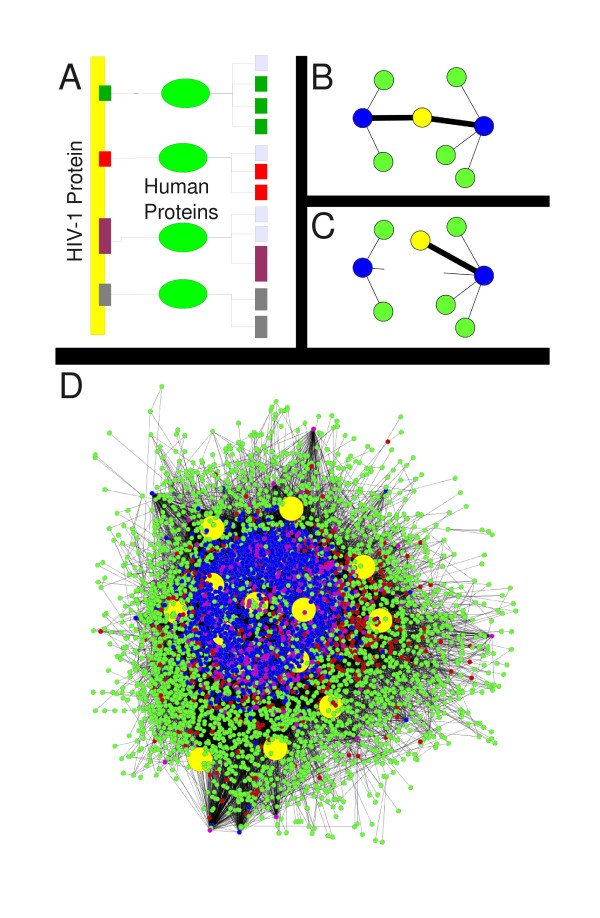
\includegraphics[scale=3.7]{figs/medGen_3}
\end{center}
\caption[Network diagrams for HIV-human protein interactions]{\small
  (A) The scheme for predicting HIV-human interactions. Rectangular
  blocks represent peptide motifs and ellipses represent the domains
  that interact with them. (B) An HIV protein (yellow) alters the
  human protein interaction network by creating a new path between
  human proteins (blue) and (C) breaking a path between two human
  proteins by competing for binding
  \cite{tournier06,sodhi04,dampier07}. (D) Here we show predicted and
  experimentally validated HIV-human interactions with the human
  interaction network (HPRD). Nodes are proteins and edges represent
  an interaction. Yellow nodes represent HIV proteins. Purple nodes
  represent the overlap between predicted (HHP) and validated (HHE)
  interactions. Blue and red nodes represent proteins specific to HHP
  and HHE, respectively, while green nodes are not involved in
  infection. \label{fig:medGen:fig3}}
\end{figure}

The prediction of HHP, the set of human proteins that might interact
with HIV proteins, was based on interactions mediated by peptide
motifs (ELMs) on virus proteins and domains (CDs) on human
proteins. We built HHP from the union of two sets of human proteins,
H1 and H2 (Figure \ref{fig:medGen:fig3}). H1 was the set of human
proteins predicted to directly interact with one or more HIV proteins
via a human CD and a virus ELM. H2 was the set of human proteins whose
interactions with proteins in H1 were potentially disrupted by
competition with an HIV protein. An H1 protein has a CD that it might
use to interact with an ELM present on both H2 and HIV proteins. For
example, in the competition between an HIV and H2 protein for
phosphorylation by an H1 kinase, the H1 protein has a kinase CD and
the competing proteins have ELMs for phosphorylation sites.

The virus-host interaction prediction algorithm was
straightforward. For each virus protein, we looked at all interactions
documented in HPRD that could be explained by an interaction between a
virus protein's conserved ELM and a CD known to interact with that
ELM, and added the protein with the CD to H1 and the protein with the
ELM to H2. To ensure that an interaction between H1 and H2 proteins
did not involve the same human protein, we removed all such self edges
from the network. Human proteins are involved in multiple protein
interactions, so H1 and H2 were not mutually exclusive. H1 contained
600 proteins, H2 contained 2151, and their intersection had 403
proteins. The total set of human proteins predicted to interact with
an HIV protein was the union of the HIV protein's H1 and H2 sets, and
contained all host proteins that were predicted to either bind to, or
compete with, the HIV protein. Across all HIV proteins, we predicted
2348 human proteins were involved in 23330 HIV-human interactions.

\subsection{Validation using the NCBI HIV-Human Protein Interaction Database}

We used the NCBI HIV-Human Protein Interaction Database (accessed
August 2008), which has 3950 interactions between 19 HIV proteins and
1439 human proteins, to evaluate our HIV-human interaction
predictions. HIV proteins ENV, GAG, and POL are cleaved into smaller
functional proteins. The NCBI database maintains different sets of
HIV-human interactions for cleavage products and the polyproteins from
which they were made. For instance, HIV POL cleavage products IN, PR,
and RT have some HIV-human interactions that are not attributed to
POL. This distinction did not work for our evaluation purposes because
under our interaction prediction method, cleavage products had a
subset of the interactions attributed to their uncleaved progenitors
because of the sequence overlap. For this reason, we took all ENV,
GAG, and POL cleavage product virus-host interactions and assigned
them to the polyprotein from which they came. When evaluating our
HIV-human interaction predictions for each HIV protein, we still
looked at interactions for GAG and POL cleavage products
individually. However, we did not assess our predictions for human
interactions with ENV cleavage products GP41 and GP120 separately from
our ENV assessment because there were so few.

We restricted the human proteins interacting with HIV proteins to
those that we could predict with our motif/domain prediction method,
i.e.\ we only looked at human proteins in the HPRD human network that
had domains and interacted with one human protein other than
itself. These restrictions left a set of 5954 host proteins that we
could predict with our algorithm. The NCBI HIV-human interactions are
spread over 68 interaction types, such as `interacts with',
`phosphorylates', and `upregulates'. We considered all interaction
types, both direct and indirect. For each HIV protein, we removed an
interaction type if it described less than six interactions. This
resulted in a set of 1,687 verified interactions between 15 HIV
proteins and 887 human proteins. We refer to this set as HHE, and used
to investigate the usefulness of our predictions. When we considered
our predicted interactions for each HIV protein individually, we only
looked at HIV proteins with more than ten interactions with human
proteins in our restricted HPRD human network, leaving twelve HIV
proteins (ENV, GAG, IN, MA, NEF, POL, PR, REV, RT, TAT, VIF, and VPR)
to consider. We constructed a subset of HHE, DHHE, which had
interaction types deemed to be direct by Tastan et
al. \cite{tastan09}. DHHE was used to evaluate the portion of our
predicted proteins that contained domains, as these proteins were more
likely to have direct interactions with HIV proteins.

%% To compare our predicted virus-host interactions with interactions
%% verified by NCBI, we looked at the overlap between virus targeted
%% proteins from both sets, KEGG pathway enrichment,

\subsubsection{Computations used for the comparison of predicted and validated HIV targeted human proteins}

To compare our predicted set of interactions with the experimentally
verified dataset from NCBI, we focused on the overlap between the two
sets, Gene Ontology (GO) \cite{ashburner00} molecular function
enrichment, GO biological process similarity, and KEGG pathway
\cite{kanehisa08} enrichment. P-values for the overlap between sets of
predicted and verified HIV targeted proteins and their various subsets
were calculated using the hypergeometric test using a background set
of 5954 possibly predicted human proteins. P-values for GO and KEGG
term enrichment for a given protein set compared to the background set
of 5954 possibly predicted human proteins were found using Bonferroni
corrected p-values from the Database for Annotation, Visualization,
and Integrated Discovery (DAVID) tool \cite{dennis03}.

To statistically compare the GO biological process similarity between
predicted and validated virus targeted proteins, we devised a
permutation test based on GO similarity between proteins, as
calculated by the GS2 tool \cite{ruths2009gs}. GO is a hierarchy of
labels, with general biological processes at the first level, and more
specific ones on higher levels. The GS2 tool takes two proteins, finds
where their GO labels are in the GO hierarchy, and calculates a
distance between all GO labels based on how far away they are in the
GO hierarchy. The GO similarity between two proteins is the average
GS2 distance between the GO labels that annotate the proteins. When we
compared predicted and validated virus targeted proteins, we limited
the comparison to only proteins with GO biological process labels in
the fifth level of the GO hierarchy. We chose this level because the
biological process labels here are specific enough for a meaningful
comparison, yet general enough to annotate large numbers of proteins
in our predicted and validated protein sets.

We performed the test for significant GO similarity between predicted
and validated HIV targeted proteins for HIV proteins with at least ten
targeted human proteins with GO labels in the fifth level of the GO
hierarchy. To find the GO similarity between predicted and validated
protein sets, we first found the GO similarity between all protein
pairs taken from the two sets, and then averaged the GO similarity for
all cross set comparisons. For the permutation test to assess the
significance of the GO similarity between predicted and validated
virus targeted protein sets, we constructed one hundred random sets of
predicted human targets for each HIV protein by sampling from a
background set of 4501 human proteins that were both considered in our
study of HPRD human network proteins, and had GO biological process
labels in the fifth level of the GO hierarchy. For each HIV protein's
GO similarity between predicted and verified human targets, we arrived
at a p-value describing the significance of the similarity by counting
the number of random predicted sets that had an equal or greater GO
similarity with the validated HIV-human interactors.

%% GO biological process similarity between predicted and validated sets
%% of HIV targeted proteins was calculated using the GS2 tool
%% \cite{ruths2009gs}, and the significance of this similarity was
%% assessed using a permutation test with one hundred random trails. In
%% each trial, we constructed a random set of predicted human virus
%% targets by sampling from the background set of 5954 human proteins
%% that had GO biological process labels. We used GO biological process
%% level 5 labels as a proxy for biological pathways, and found the
%% average GO similarity for all predicted/validated gene pairs taken
%% from HHP and HHE \cite{ruths2009gs}. For each HIV protein, we compared
%% the resulting average GO similarity between HHP and HHE to 100 random
%% scores made by sampling HHP sets from the HPRD background.

\section{Results}

\subsection{Human peptide motifs were conserved on HIV proteins}

\begin{figure}
\begin{center}
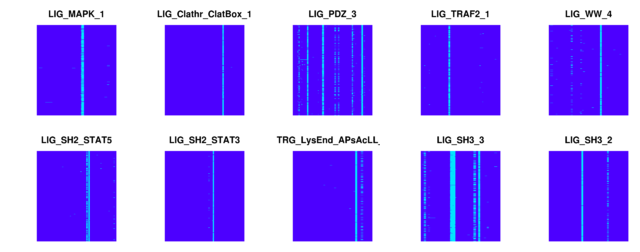
\includegraphics[scale=.5]{figs/medGen_1}
\end{center}
\caption[Host peptide motif conservation on HIV NEF]{\small This
  figure shows host peptide motif conservation on NEF. Peptide motifs
  (ELMs) were spatially conserved on alignments of HIV proteins of
  subtypes B and C. Each box shows the annotations for one conserved
  ELM (present on more than 70\% of protein instances) on the multiple
  alignment of NEF protein sequences taken from different patients. An
  ELM can be spatially conserved in multiple positions on the
  alignment, demonstrated by multiple sets of thick vertical lines in
  an ELM's box. \label{fig:medGen:fig1}}
\end{figure}

Figure \ref{fig:medGen:fig1} shows a subset of the conserved peptide
motifs (ELMs) annotated on HIV NEF's multiple protein sequence
alignment. It is clear from the figure that conserved ELMs occur in
roughly the same position on each aligned protein. Our computations
showed that this was true for all conserved ELMs on all HIV
proteins. The HIV reverse transcription process is susceptible to
errors, with HIV RT making roughly 0.2 errors per genome in each
replication cycle \cite{rambaut2004causes}, which leads to an
evolutionary rate one million times that of host genomes
\cite{mansky1998retrovirus}. Noting that HIV is a virus with high
mutation rate, it is likely that conserved ELMs are essential for
viral replication within the host cell \cite{kadaveru08}. ELM
annotation in eukaryotic proteomes is not yet complete. Multiple
computational strategies have been employed for the discovery of
additional ELMs involved in protein interactions and
post-translational modifications \cite{neduva06biotech,dinkel07}. It
is possible that HIV proteins have additional conserved ELMs that have
not yet been identified.

\begin{figure}
\begin{center}
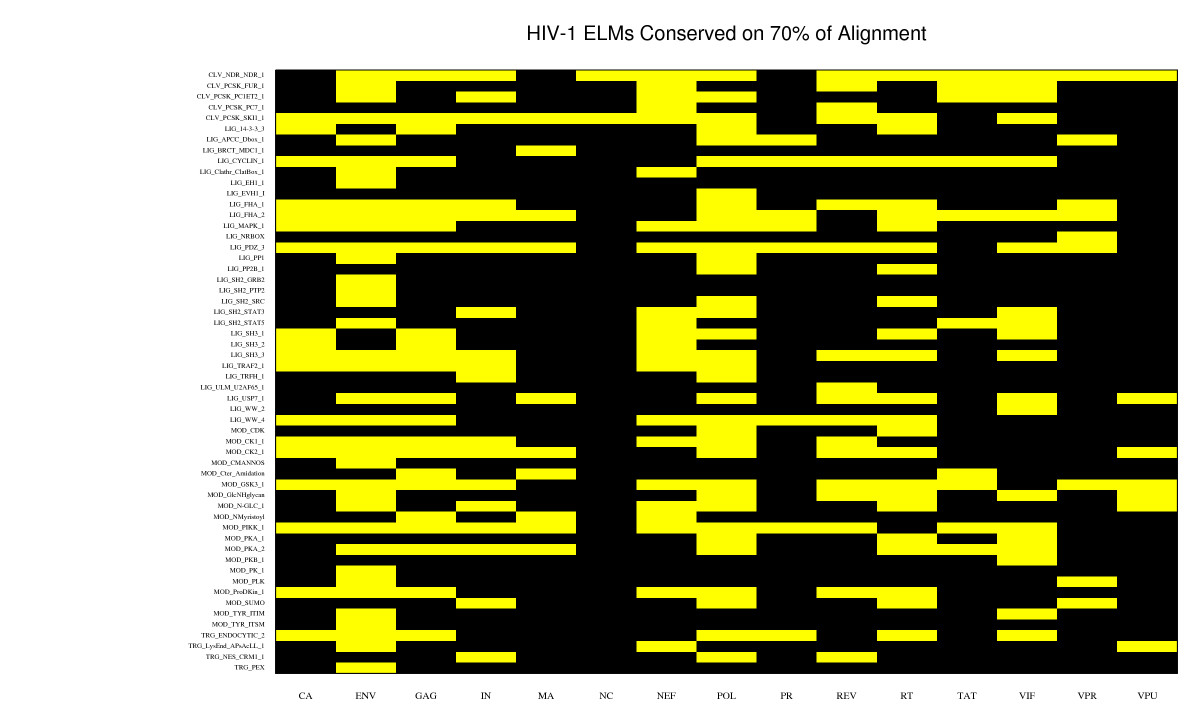
\includegraphics[scale=2]{figs/medGen_2}
\end{center}
\caption[Host peptide motifs conserved on HIV proteins]{\small Here we
  show conserved host peptide motifs (ELMs) on HIV proteins. Of 133
  ELMs scanned, only 56 were conserved (present on more than 70\% of
  an HIV protein's sequence alignment). Yellow boxes indicate
  conservation of an ELM above 70\% for a virus protein. All HIV
  proteins shown had at least one conserved
  ELM. \label{fig:medGen:fig2}}
\end{figure}

Conserved peptide motifs (ELMs) are shown for each HIV protein in
Figure \ref{fig:medGen:fig2}. Overall, 56 of the 133 ELMs in the ELM
Resource were conserved on some HIV protein. Some of the conserved
ELMs, like the SH3 ligand sites on NEF, have been experimentally
verified as binding sites for human proteins \cite{coleman06}. We
found that some conserved ELMs occur frequently on human proteins. A
PDZ domain binding site, ELM LIG\_PDZ\_3, was seen on 90\% of human
proteins. Other ELMs, like LIG\_EH1\_1, a binding site for the WD40
domain, appeared on only a few human proteins (see Supplemental table
\ref{tbl:medGenAdd1:counts}).

%% To see if ELM conservation on HIV protein alignments was occurring by
%% chance, we generated random HIV NEF protein sequences and annotated
%% them with ELMs (see Methods). We found that

\subsection{Significant overlap of predicted and validated HIV-human interactions verifies our method}

The NCBI set of curated HIV-human interactions contains 887 host
proteins known to interact with one or more HIV proteins. The dataset
captures both direct and indirect, regulatory HIV-human protein
interactions \cite{fu09}, and was appropriate for the task of
assessing our predicted interactions because it allowed us to judge
our algorithm's ability to capture both direct and indirect
interactions. The HPRD human protein interaction network containing
the 5954 human proteins in this study is shown in Figure
\ref{fig:medGen:fig3}D with yellow HIV proteins connected to their
predicted interaction partners (blue) and their verified interaction
partners (red). Proteins in both sets are purple, while all other
proteins are green. As seen in the figure, our predicted set of virus
targeted human proteins, with over two thousand proteins, was larger
than the verified NCBI list, with only 877 proteins. 



\begin{table}\footnotesize
\begin{center}
  \begin{tabular}{|l|c|c|c|c|}
  \hline
  HIV protein & HHP & HHE & Overlap & P-value \\
  \hline
%CA&     1878&   7&      1&      7.02e-01\\
ENV&    2166&   409&    194&    8.09e-07\\
GAG&    2035&   103&    46&     9.94e-03\\
IN&     1759&   46&     12&     0.631\\
MA&     1129&   47&     19&     1.60e-04\\
%NC&     9&      7&      0&      1.00e+00\\
NEF&    1828&   155&    83&     6.42e-10\\
POL&    2093&   122&    57&     2.96e-03\\
PR&     1169&   58&     20&     2.30e-03\\
REV&    1702&   40&     16&     4.11e-02\\
RT&     1986&   23&     20&     1.07e-08\\
TAT&    1106&   509&    183&    5.54e-23\\
VIF&    1832&   35&     7&      0.888\\
VPR&    919&    119&    39&     5.29e-07\\
%VPU&    164&    7&      1&      1.45e-02\\
\hline
  \end{tabular}
\end{center}
\caption[Overlap between predicted and validated HIV-human
  interactions]{\small For each HIV protein, we evaluated the
  significance of the overlap between human proteins in HIV-human
  predicted and validated interactions. The HHP column gives the
  number of human proteins that were predicted to interact with an HIV
  protein, while HHE shows the number of verified virus targeted
  proteins in the NCBI database. The Overlap column counts the number
  of proteins in both sets. P-values for the overlap between predicted
  and validated HIV targeted proteins were calculated using a
  hypergeometric test (see Methods). We limited our results to HIV
  proteins with at least ten verified interactions with human
  proteins. \label{tbl:medGen:eval}}
\end{table}


For a more quantitative evaluation of our predictions, we compared
predicted and verified HIV targeted proteins for all HIV proteins
individually. The significance of the overlap between predicted and
verified interactions is shown in Table \ref{tbl:medGen:eval}. Of the
twelve virus-host predicted interaction sets we evaluated, only two,
from HIV proteins IN and VIF, did not have significant overlap with
the NCBI interactions. While the overlap between predicted and
validated interactions was significant (p-value $<$ 0.05), and the
recall of known virus-host interactions for each HIV protein was at
least 20\%, there were many predicted interactions that were not
validated by the NCBI database. 

Our predicted interactions consisted of human proteins with domains
that interact with conserved HIV peptide motifs (H1 proteins), and
human proteins that that interacted with H1 proteins and were
annotated with HIV peptide motifs (H2 proteins). Proteins in H2
dominated the overlap between predicted and validated virus targeted
proteins. Roughly two thirds of the proteins in H1 were also found in
H2. For this reason, we sought to evaluate H1 separately from our
total prediction set. For each HIV protein, we investigated the
usefulness of H1 by comparing it with DHHE, the validated NCBI direct
virus-host interactions. We limited our comparisons to the twelve HIV
proteins with at least ten direct interactions with human proteins,
and found that eight of these HIV proteins (ENV, GAG, MA, NEF, POL,
REV, RT, and TAT) had significant overlap between H1 and DHHE (see
Supplemental table \ref{tbl:medGenAdd3:direct}). Figure
\ref{fig:medGen:fig4} shows the overlap p-values and sizes of DHHE and
H1 for HIV proteins ENV, NEF, and TAT. Our H1 predictions for HIV
proteins IN and VIF failed to have significant overlap with validated
direct interactions, just as our full set of predicted interactions for
these HIV proteins did not have significant overlap with all verified
virus-host interactions (Table \ref{tbl:medGen:eval}). While for the
HIV RT protein, H1 predictions performed better than the full
prediction set (HHP), this was not the case for the other HIV
proteins. For both H1 and HHP prediction sets, our precision was not
high, indicating that most proteins predicted to interact with HIV
were not verified by the NCBI database. For this reason, we turned to
the Gene Ontology and the KEGG pathway databases for an understanding
of how our unverified predictions captured the host cell biological
pathways and functions targeted by HIV proteins.

%% To further investigate our direct predicted interactions, we limited
%% our predicted proteins those in the KEGG pathway database
%% \cite{kanehisa08}, assuming that these proteins would have a higher
%% chance of showing up the the NCBI literature curated HIV-human
%% interactions. The upper half of 

\begin{figure}
\begin{center}
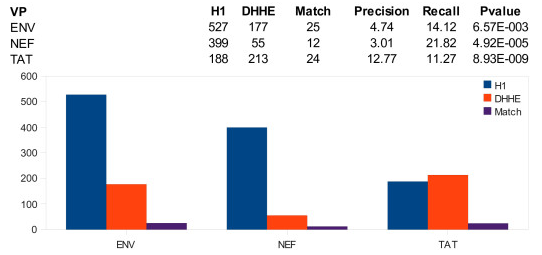
\includegraphics[scale=.75]{figs/medGen_direct}
\end{center}
\caption[Evaluation of direct HIV-human interaction
  predictions]{\small Here we compare predicted and validated
  virus-host direct interactions for HIV proteins ENV, NEF, and
  TAT. The Match column holds the overlap between predicted and
  verified virus targeted host protein sets. The figure compares host
  proteins from direct interaction predictions (H1) with host proteins
  from experimentally verified direct interactions (DHHE). The
  p-values indicated a significant overlap for all protein
  sets. P-values were calculated as described in
  Methods. \label{fig:medGen:direct_eval}}
\end{figure}

%% While the overlap we significant, recall and precision were poor, so
%% we next compared predicted and validated virus-host interactions in a
%% biological context. While we might have missed the exact interactions
%% for HIV proteins, we might have been close to them in terms of
%% molecular function and biological pathways.

\subsection{Predicted and validated HIV-human interactions share similar Gene Ontology labels}

\begin{table}\footnotesize
\begin{center}
  \begin{tabular}{|l|c|c|c|}
  \hline
  Gene Ontology Label & ENV HHP/HHE & NEF HHP/HHE & TAT HHP/HHE\\
  \hline
adenyl ribonucleotide binding  &  6.82e-12/0.003   &     NA /NA & NA/NA\\
inositol or PI kinase activity  & 7.22e-07/0.0009 &  NA/NA   &   1.033e-06/0.0016\\
lipid kinase activity   & 7.22e-07/0.0009   &    NA/NA &     2.06e-08/0.0016 \\
MAP kinase activity  &   0.00029/2.33e-07   &    NA/NA  &    NA/NA\\
phosphoinositide 3-kinase activity  &    0.0002/0.0001  &     NA/NA  &     1.54e-05/0.000167 \\
protein kinase activity & 5.60e-34/0.00085    &    2.04e-29/0.00044    &    1.01e-36/0.0035\\
protein kinase binding  & NA/NA  &    NA/NA   &   2.16e-18/3.46e-06\\
\hline
  \end{tabular}
\end{center}
\caption[Gene Ontology molecular function enrichment for predicted and
  experimentally verified HIV targeted human proteins]{\small Here we
  show Gene Ontology molecular function level 5 labels statistically
  enriched (p-value $<$ 0.01) on human proteins from our predicted
  virus-host interactions (HHP) for HIV ENV, NEF, and TAT. Enrichment
  for host proteins involved in NCBI's verified virus-host
  interactions (HHE) is also indicated.\label{tbl:medGen2:GO}}
\end{table}


As a biological validation of our results, we compared our predicted
and validated HIV-human interactions using Gene Ontology (GO) labels
of molecular function and biological process. While our predictions
missed some of the exact interactions with HIV proteins, they might
have been close to them in terms of molecular function and biological
pathways. GO labels are organized hierarchically, with general labels
towards the first levels of the hierarchy, and specific labels at the
higher levels. For our investigations, we focused on specific terms on
the fifth level of the GO hierarchy. We examined GO labels for
predicted and validated virus-host interactions for HIV proteins ENV,
NEF, and TAT because they had the most verified experimental
interactions with human proteins. First, we found the GO molecular
function level 5 labels that were enriched in our predicted virus
targeted human proteins, and then calculated the enrichment for the
host proteins in the validated NCBI HIV-human interactions. Table
\ref{tbl:medGen2:GO} shows that GO molecular functions for which our
prediction's host proteins were significantly enriched (p-value $<$
0.01) were also enriched in validated HIV targets.

\begin{table}\footnotesize
\begin{center}
  \begin{tabular}{|l|c|c|c|c|}
  \hline
  HIV protein & GO HHP & GO HHE & P-value \\
  \hline
%CA  &    1410  &  4 & 0.00 \\
ENV   &  1640  &  347 & 0.00 \\
GAG  &   1545  &  88 & 0.00 \\
IN   &   1347 &   44 & 0.99 \\
MA  &    872  &   45 & 0.00 \\
%NC  &    7    &   6 & 0.19 \\
NEF &    1376 &   126 & 0.00 \\
POL &    1595 &   116 & 0.00 \\
PR  &    882  &   54 & 0.00 \\
REV  &   1273 &   35 & 0.00 \\
RT  &    1517 &   23 & 0.00 \\
TAT  &   857  &   445 & 0.00 \\
VIF  &   1397 &   32 & 0.98 \\
VPR  &   694  &   93 & 0.00 \\
%VPU  &   124  &   6 & 0.06 \\

%CA & H1 & 0.20 \\
%CA & 0.00 \\
%ENV & H1 & 0.00 \\
%ENV & 0.00 \\
%GAG & H1 & 0.00 \\
%GAG & 0.00 \\
%IN & H1 & 0.76 \\
%IN & 0.99 \\
%MA & H1 & 0.00 \\
%MA & 0.00 \\
%NC & H1 & 0.44 \\
%NC & 0.19 \\
%NEF & H1 & 0.03 \\
%NEF & 0.00 \\
%POL & H1 & 0.00 \\
%POL & 0.00 \\
%PR & H1 & 0.02 \\
%PR & 0.00 \\
%REV & H1 & 0.03 \\
%REV & 0.00 \\
%RT & H1 & 0.00 \\
%RT & 0.00 \\
%TAT & H1 & 0.00 \\
%TAT & 0.00 \\
%VIF & H1 & 0.21 \\
%VIF & 0.98 \\
%VPR & H1 & 0.19 \\
%VPR & 0.00 \\
%VPU & H1 & 1.00 \\
%VPU & 0.06 \\
\hline
  \end{tabular}
\end{center}
\caption[Validation of HIV-human predicted interactions using Gene
  Ontology biological process similarity]{\small For each HIV protein,
  we evaluated the performance of our HIV-human interaction
  predictions (HHP) using Gene Ontology (GO) biological process labels
  to compare our predicted interactions to experimentally validated
  interactions. We computed a GO similarity score between predicted
  and validated protein sets by averaging over all GO similarity
  scores that resulted from pairwise combinations of proteins taken
  from the predicted and validated protein sets (see Methods). For
  each HIV protein, we constructed random HHP sets to use in a
  permutation test to evaluate the significance of the observed GO
  similarity between HHP and HHE. We report the p-values for these
  trials.

%% We further compared our direct predicted interactors (H1) and our
%% total prediction set (HHP) with the experimentally validated
%% interctions using GO biological process level 5 terms. For each
%% prediction and validation set, we calculated the similarity in GO BP 5
%% annotations, and then used a permutation test with 100 trials to
%% evaluate the significance of the observed score. We report the
%% p-values for these trials. 
\label{tbl:medGen3:GOsim}}
\end{table}


For a more quantitative assessment of our predicted HIV-host
interactions, we measured the similarity between predicted HIV
targeted pathways and known HIV targeted pathways, using GO biological
process level 5 labels as a proxy for pathway annotations. For each
HIV protein, we computed the average GO similarity for all
predicted/validated protein pairs taken from host proteins in
predicted and validated virus-host interactions, and found the
significance of the GO similarities using a permutation test (see
Methods). Table \ref{tbl:medGen3:GOsim} shows that predictions for
most HIV proteins had significant GO similarity with verified virus
targeted proteins. Just as predictions of virus-host interactions for
HIV proteins IN and VIF did not show a significant overlap with
verified interactions, the GO similarities between predicted and
verified virus-host interactions for these HIV proteins were not found
to be statistically significant. For the other HIV proteins, it is
likely that some of our unverified predictions from Table
\ref{tbl:medGen:eval} and Figure \ref{fig:medGen:direct_eval} are
correct, or have some importance for HIV infection, because they act
in the same biological processes that HIV targets.

\subsection{Predicted and validated HIV-human interactions occupy the same KEGG pathways}

\begin{table}\footnotesize
\begin{center}
  \begin{tabular}{|l|c|c|c|}
  \hline
  KEGG Pathway & ENV HHP/HHE & NEF HHP/HHE & TAT HHP/HHE\\
  \hline
AML & 1.97E-05/2.68E-05 & 2.07E-05/8.55E-05 & 2.66E-08/3.08E-04 \\
Adherens junction & 2.15E-09/NA & 8.21E-11/NA & 6.74E-06/NA \\
Apoptosis & 4.58E-04/1.43E-13 & 5.18E-04/6.54E-04 & 3.91E-03/3.88E-13 \\
B cell receptor signaling & 4.86E-06/8.73E-10 & 2.88E-04/2.90E-04 & 1.25E-09/5.57E-06 \\
Cell cycle & NA/NA & NA/NA & 2.88E-04/1.90E-01 \\
CML & 7.21E-05/2.23E-05 & 1.17E-06/2.46E-05 & 1.01E-09/7.53E-07 \\
Colorectal cancer & 1.07E-05/3.18E-04 & 4.68E-08/3.31E-03 & 4.50E-04/1.42E-03 \\
Endometrial cancer & 6.03E-04/1.62E-02 & 1.66E-04/2.10E-03 & 5.03E-07/3.83E-04 \\
Signaling in H. pylori infection & 2.29E-04/3.84E-06 & 2.07E-06/2.83E-05 & NA/NA \\
ErbB signaling & 2.27E-10/5.70E-04 & 1.70E-12/9.22E-04 & 1.53E-12/1.66E-05 \\
Fc epsilon RI signaling & 8.43E-04/6.23E-21 & 2.14E-05/2.20E-07 & 9.62E-05/1.52E-04 \\
Focal adhesion & 2.82E-06/2.30E-03 & 2.31E-07/6.90E-02 & 5.28E-08/3.36E-09 \\
Gap junction & 1.90E-04/1.26E-04 & NA/NA & 1.12E-04/7.18E-10 \\
Glioma & 1.50E-04/1.24E-05 & 4.99E-06/6.02E-03 & 1.56E-07/6.79E-11 \\
Insulin signaling & 1.53E-07/8.84E-02 & 1.73E-04/3.50E-01 & 2.91E-07/7.35E-02 \\
Jak-STAT signaling & 4.08E-08/2.15E-04 & 4.09E-09/1.28E-01 & 2.32E-17/4.91E-03 \\
Leukocyte migration & 1.94E-07/2.21E-08 & 1.17E-08/6.36E-01 & 3.28E-05/1.45E-01 \\
Long-term potentiation & 6.79E-05/2.20E-02 & NA/NA & 9.04E-03/2.38E-10 \\
MAPK signaling & 5.19E-08/6.32E-04 & 1.58E-09/3.27E-03 & 1.18E-03/5.15E-01 \\
NK cell mediated cytotoxicity & NA/NA & NA/NA & 9.50E-06/5.31E-15 \\
Non-small cell lung cancer & 4.28E-05/1.25E-04 & 1.26E-05/1.67E-03 & 7.55E-06/1.45E-06 \\
Pancreatic cancer & 1.26E-04/5.54E-07 & 1.10E-05/2.50E-06 & 1.03E-05/8.15E-08 \\
Pathogenic E. coli infection & 3.77E-03/1.00E+00 & 2.94E-03/NA & 9.74E-03/3.25E-01 \\
Phosphatidylinositol signaling & 1.36E-03/1.72E-04 & 2.37E-03/NA & 2.19E-05/9.74E-06 \\
Prostate cancer & 1.90E-04/1.26E-04 & 6.26E-06/6.56E-05 & 5.46E-09/1.11E-07 \\
Regulation of cytoskeleton & 4.30E-03/6.02E-01 & 1.73E-03/8.79E-01 & 2.66E-03/7.65E-01 \\
Small cell lung cancer & 1.94E-03/3.71E-10 & 8.42E-05/4.25E-02 & 1.12E-04/4.09E-14 \\
T cell receptor signaling & NA/NA & NA/NA & 1.56E-06/1.35E-11 \\
Tight junction & 1.24E-03/1.00E+00 & 5.29E-04/NA & NA/NA \\
Toll-like receptor signaling & 5.16E-03/2.04E-14 & 5.37E-05/2.04E-14 & NA/NA \\
Type II diabetes mellitus & NA/NA & NA/NA & 3.47E-03/5.95E-01 \\
VEGF signaling & 3.23E-03/4.89E-15 & 6.79E-03/8.82E-03 & 1.88E-05/4.07E-12 \\
\hline
  \end{tabular}
\end{center}
\caption[KEGG pathway enrichment for predicted and experimentally
  verified HIV targeted human proteins]{\small Here we show KEGG
  pathways enriched (p-value $<$ 0.01, see Methods) with human proteins
  from our predicted virus-host interactions (HHP) for HIV ENV, NEF,
  and TAT. Enrichment for host proteins involved in NCBI's verified
  virus-host interactions (HHE) is also
  indicated. \label{tbl:medGen1:KEGG}}
\end{table}


Since our predicted virus-host interactions performed well at
recovering known HIV targeted biological processes, we moved to an
evaluation of our predictions that involved more defined biological
pathways from the KEGG pathway database. The KEGG pathways
statistically enriched for HIV ENV, NEF, and TAT interacting proteins
(experimental as well as computational) included immune system
pathways such as T cell and B cell receptor signaling pathways,
apoptosis, focal adhesion, and toll-like receptor signaling pathways
(Table \ref{tbl:medGen1:KEGG}). Gene expression data before and after
HIV infection of macrophages also showed apoptosis and MAPK signaling
pathways as statistically enriched \cite{brown08}, as predicted
here. Microarray results did not show cell cycle and toll-like
receptor pathways as highly activated in HIV activated macrophages,
although the toll-like receptor pathway was highly enriched with known
HIV targeted proteins (Table \ref{tbl:medGen1:KEGG}). Also
statistically enriched were disease pathways such as the colorectal
cancer, leukemia, and lung cancer pathways that have been shown to
have high incidence of occurrence in HIV infected individuals
\cite{patel08}. Other disease pathways predicted by our analysis
included those previously associated with HIV infection: H. pylori
infection \cite{panos07}, E. coli infection \cite{ramakrishna99}, and
type II diabetes \cite{panz99}. These observations indicated the
promise of our method in predicting activated disease pathways based
on viral sequence. Post-translational modification appeared to be an
important element of HIV cellular network hijacking. As shown in Table
\ref{tbl:medGen2:GO}, protein kinase activity and protein kinase
binding were significantly enriched both in predicted and verified HIV
targeted proteins, suggesting the importance of altered
phosphorylation events in the reorientation of the host cell
interaction network towards virus survival and replication
\cite{brown08}. The HIV activated GO categories listed in Table
\ref{tbl:medGen2:GO} are associated with signal transduction processes
in the KEGG pathways presented in Table \ref{tbl:medGen1:KEGG}.

\begin{figure}
\begin{center}
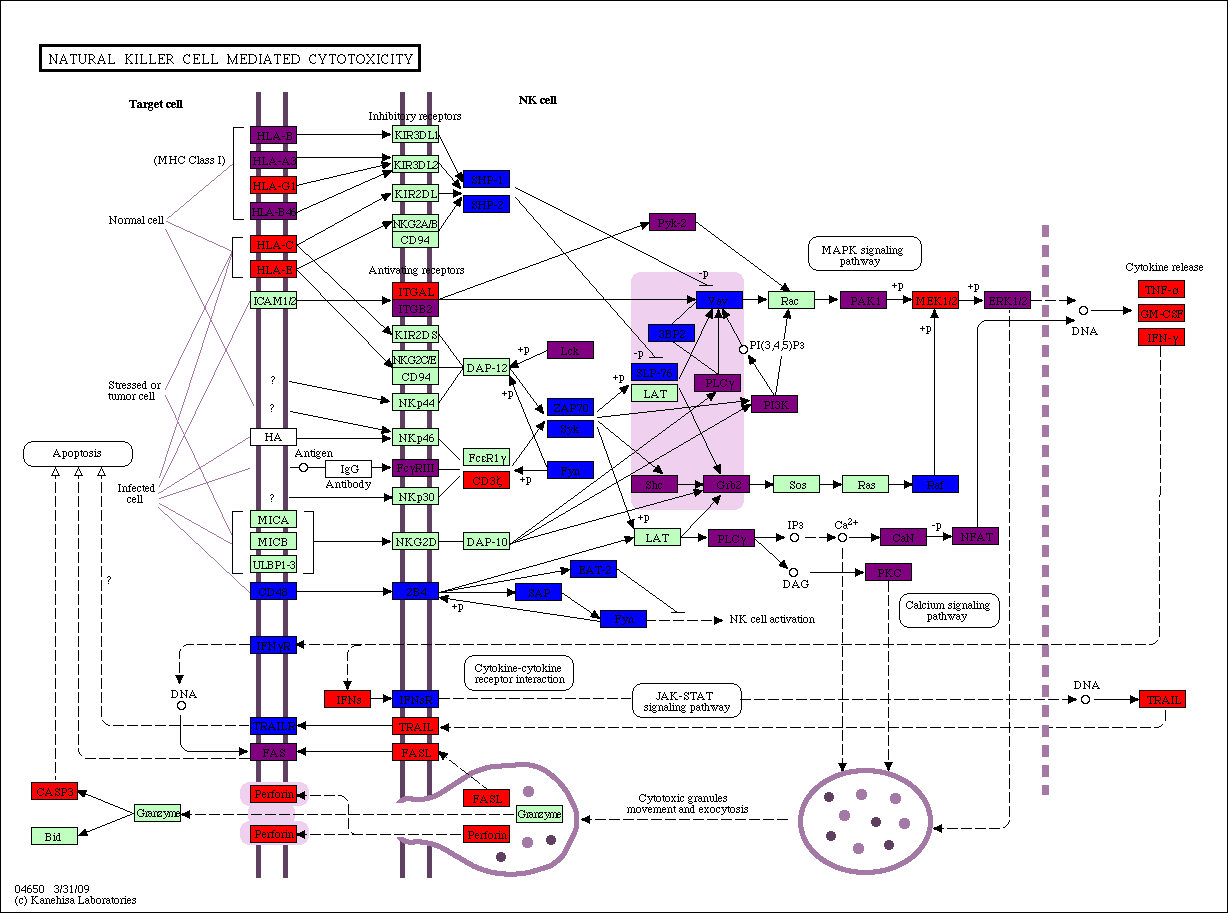
\includegraphics[scale=0.25]{figs/medGen_5}
\end{center}
\caption[HIV TAT natural killer cell mediated cytotoxicity]{\small HIV
  TAT natural killer cell mediated cytotoxicity. The KEGG natural
  killer cell mediated cytotoxicity pathway is colored for predicted
  TAT-human interactions (blue) and validated TAT-human interactions
  (red), and their overlap (purple). Green boxes have proteins not
  involved in infection, while white boxes do not have human
  proteins. \label{fig:medGen:fig5}}
\end{figure}

The positions of predicted and matched HIV targeted proteins along
KEGG pathways allowed us to assess the overlap between computational
and experimental prediction based on cell-compartment identity. Figure
\ref{fig:medGen:fig5} shows the overlap (purple) between predicted
(blue) and experimentally determined (red) host proteins targeted by
HIV TAT along the natural killer cell mediated cytotoxicity
pathway. Our predictions were on target on the cell membrane for
HLA-B, HLA-A3, HLA-B45, and FAS, but we missed Perforin, HLA-C, HLA-E,
and HLA-G1. The figure also shows a good match for DNA transcription
factors targeted by HIV. The green boxes in the figure correspond to
host proteins with apparently no direct interaction with TAT.

\begin{figure}
\begin{center}
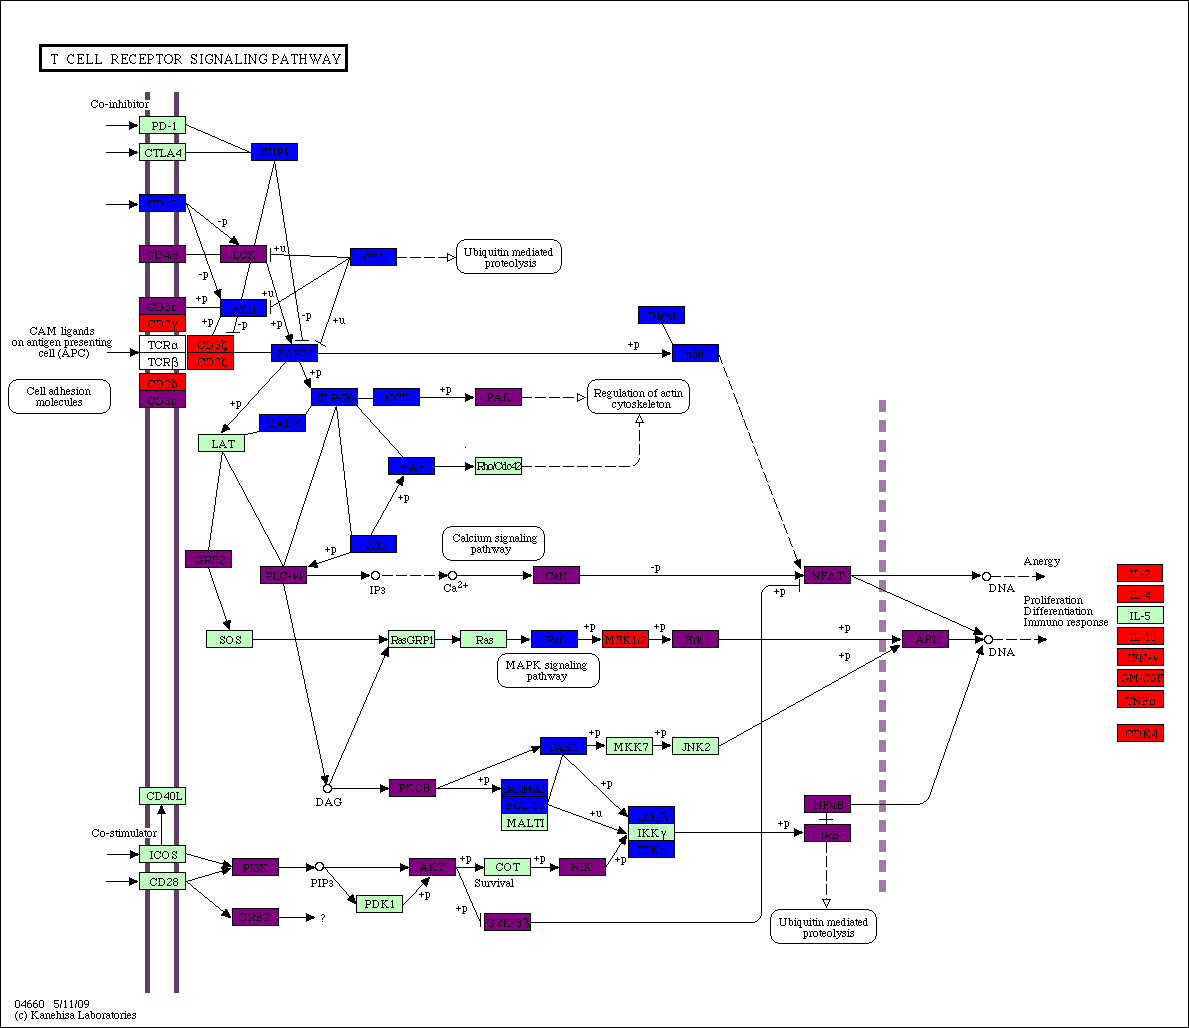
\includegraphics[scale=0.25]{figs/medGen_6}
\end{center}
\caption[HIV TAT T cell receptor signaling pathway]{\small HIV TAT T
  cell receptor signaling pathway. The KEGG T cell receptor signaling
  pathway is colored for predicted TAT-human interactions (blue) and
  validated TAT-human interactions (red), and their overlap
  (purple). Green boxes have proteins not involved in infection, while
  white boxes do not have human proteins. \label{fig:medGen:fig6}}
\end{figure}

The cytokines shown in red at the right hand side of the KEGG diagram
in Figure \ref{fig:medGen:fig5} would not be expected to appear in our
predicted list. They are documented in the NCBI database as interacting
with HIV, but their interactions with virus proteins are probably not
direct, but via transcriptional regulation. The T cell receptor
signaling pathway in Figure \ref{fig:medGen:fig6} had a high degree of
overlap (purple) along the cell membrane and on transcription factors
between TAT targeted host proteins (red) and our corresponding
predictions (blue). The abundance of predicted host proteins in the
pathway with no matching experimental result suggested new virus-host
interaction studies for HIV as well as a justification for further
refinement of our computational method, perhaps by incorporating
protein structures \cite{doolittle2010structural}.

%%  Since our predictions might be used in this way,
%% we decided to evaluate only our predictions that were present in KEGG
%% pathways.

 %% We found KEGG pathways
%% enriched with proteins from each virus protein's predicted interaction
%% partners (p-value $<$ 0.01, see Methods).

Human proteins in our predicted HIV-human interactions performed well
at capturing virus-targeted KEGG pathways. One reason that this
pathway evaluation showed our predictions to be more promising than a
simple protein set comparison could be that proteins in KEGG pathways
are better studied than proteins in the HPRD human interaction network
\cite{kanehisa08}. We attempted to obtain a set of predicted
interactions with fewer false positives by limiting human proteins in
our predicted interactions to those that were in KEGG pathways. We
then compared the overlap between KEGG restricted predicted virus-host
interactions and validated virus-host interactions for HIV proteins
ENV, NEF, and TAT (Figure \ref{fig:medGen:fig4}). We found that the
intersection between predicted and verified virus-host interactions
for human proteins in the HPRD human interaction network became more
significant as we limited predictions to proteins in KEGG pathways
(Figure \ref{fig:medGen:fig4} and Supplemental table
\ref{tbl:medGenAdd4:kegg}). Restricting predictions to all KEGG
pathways produced a set of virus-host interactions with less false
positives, so we decided to restrict our predictions further by
finding KEGG pathways that were enriched with human proteins from
predicted HIV-human, and keeping only predictions in these pathways.

Viruses often target specific host pathways, like the type I
interferon response pathway, and interact with multiple host proteins
in these pathways \cite{navratil-system,yeung09}. We hypothesized that
estimating HIV targeted pathways from our predicted virus-host
interactions, and then restricting our predictions to only human
proteins in these pathways would yield better results than limiting
our predictions to all KEGG pathways. We were further motivated to
find KEGG pathways enriched with our predictions because studying
proteins in specific pathways is valuable because predicted
interactions with certain pathways can be used to guide targeted
virus-host interaction experiments \cite{lee2004probabilistic}. We
limited our predicted interactions by focusing on human proteins in
KEGG pathways that were found to be enriched with our predictions
(p-value $<$ 0.01, see Methods). Bar graphs in Figure
\ref{fig:medGen:fig4} demonstrate the intersection of predictions when
restricted to the KEGG pathways in which they are enriched with
verified interactions for HIV ENV, NEF, and TAT. Compared to limiting
our predictions to proteins in all KEGG pathways, restricting
predictions for HIV ENV and NEF to proteins in KEGG pathways that were
statistically enriched with human proteins in our virus-host
prediction for these HIV proteins (p-value $<$ 0.01) improved the
overlap between predicted and verified virus-host interactions.

%% The p-values indicated a statistically significant match between
%% predicted and experimental sets for ENV, NEF, and TAT when using both
%% direct predictions (H1), and direct predictions in addition to
%% competing predictions (HHP). However, the p-values in Figure
%% \ref{fig:medGen:fig4} showed that the overlap between predicted and
%% experimental data was weaker for H1 and DHHE than for HHP and HHE.

\begin{figure}
\begin{center}
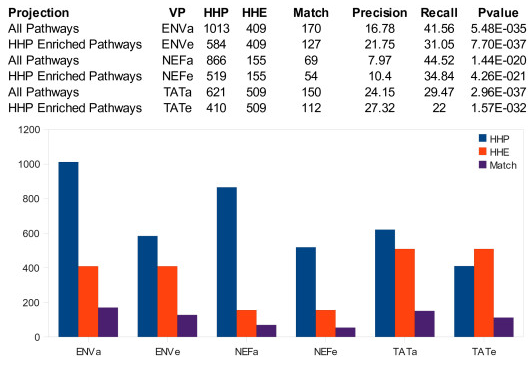
\includegraphics[scale=.75]{figs/medGen_kegg}
\end{center}
\caption[Comparison of predicted and validated virus-host interactions
  for host proteins in KEGG pathways]{\small Here we compare predicted
  and validated virus-host interactions for host proteins in KEGG
  pathways. The Match column holds the overlap between predicted and
  verified virus targeted host protein sets. The figure compares host
  proteins from all predicted (HHP) and verified (HHE) interactions
  for the three HIV proteins. Predicted host proteins were restricted
  to either genes in all KEGG pathways (ENVa, NEFa, TATa), or KEGG
  pathways enriched (p-value $<$ 0.01, see Methods) with our
  predictions (ENVe, NEFe, TATe). The intersection between predicted
  and verified interactions was significant for both restrictions, but
  slightly more significant for enriched pathways for HIV proteins ENV
  and NEF. P-values were calculated as described in
  Methods. \label{fig:medGen:fig4}}
\end{figure}

%% One reason that the pathway evaluation showed our predictions to be
%% more promising than a simple protein set comparison is that proteins
%% in KEGG pathways are well studied. To obtain a better set of
%% predictions, we limited our human proteins in our predicted
%% interactions to those that were in KEGG pathways.

%% Proteins in KEGG are better studied than proteins in HPRD
%% \cite{kanehisa08}. 

%% One potential contributor to such low
%% p-values is that host proteins in KEGG pathways are among the most
%% studied, and therefore their interactions with HIV proteins would have
%% been investigated earlier than the poorly studied host
%% proteins. Nevertheless, the correspondence between statistically
%% enriched HHP and HHE KEGG pathways (Table \ref{tbl:medGen1:KEGG},
%% p-value $<$ 0.01) and the enriched GO molecular function level 5
%% labels (Table \ref{tbl:medGen2:GO}, p-value $<$ 0.01), suggested the
%% co-localization of HHP and HHE in the host proteome.

\begin{figure}
\begin{center}
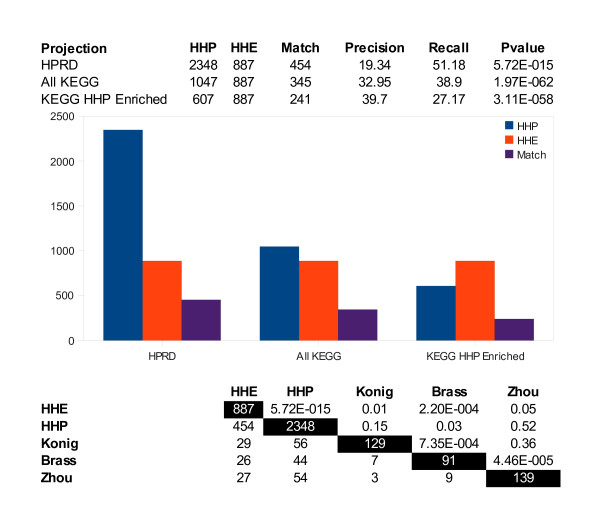
\includegraphics[scale=2.25]{figs/medGen_7}
\end{center}
\caption[Comparison of combined predicted and validated virus-host
  interactions]{\small Here we evaluate our predictions on the virus
  level, rather than the virus protein level. For both predicted and
  validated virus-host interactions, we combined the host targets of
  individual HIV proteins to produce virus level protein sets. The
  overlap (Match) of our predictions (HHP) with verified HIV targeted
  proteins (HHE) was compared when restricting them to proteins in
  HPRD, KEGG, and KEGG pathways enriched in HHP (p-value $<$ 0.01, see
  Methods). The lower table compares HHE, HHP, and predictions from
  three siRNA screens. The darkened diagonal holds the sizes of all
  sets. The overlap between sets is below the diagonal, while p-values
  for these overlaps are above (see Methods). \label{fig:medGen:fig7}}
\end{figure}

\subsection{Virus level comparison of predicted and verified HIV-human interactions}

We have evaluated our predicted interactions for individual HIV
proteins, but another way to view our predictions is at the virus
level. At the virus level, we can check to see if human proteins that
were predicted to interact with one HIV protein have any validated
interactions with other HIV proteins. This test was motivated by the
observation that virus proteins often interact with the same host
proteins \cite{ptak08}. Figure \ref{fig:medGen:fig7} shows a combined
view of predicted and validated virus-host interactions, made by
aggregating interactions for all virus proteins. When we restricted
our predictions to KEGG proteins, we had 1047 host proteins, and 345
of these had already been shown to be interacting with at least one
HIV protein. The match between computational prediction and
experimental data in this case led to a p-value of 1.97e-62. The
improvement seen in recall and precision for virus level predictions
compared to HIV protein level predictions indicated that our
predictions captured many of the host interactions shared between HIV
proteins, and that interaction predictions made for one virus protein
could be used to capture interactions with other HIV proteins.

%% One reason for the small
%% p-value is that a host protein was considered to be interacting with
%% HIV even if the protein interacted with an HIV protein other than the
%% one that was experimentally verified. Nevertheless, this virus protein
%% insensitive set is meaningful, as it provides a first estimate of HIV
%% targeted host proteins.

\subsection{Infrequent host peptide motifs did not improve prediction performance}

\begin{figure}
\begin{center}
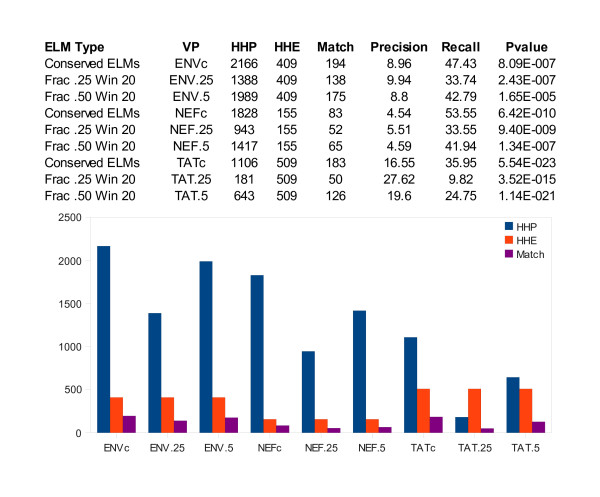
\includegraphics[scale=2]{figs/medGen_8}
\end{center}
\caption[Evaluating the use of infrequent host peptide motifs for
  HIV-human interaction prediction]{\small Here we tested the
  hypothesis that using infrequent host peptide motifs for HIV-human
  interaction prediction, rather than all host peptide motifs
  conserved on HIV proteins improved the performance of our
  predictions. We found infrequent host peptide motifs by limiting
  conserved HIV peptide motifs to those that occurred on less than some
  fraction (Frac) of human proteins, or were seen on an HIV protein
  with another peptide motif within a twenty residue window, resulting
  in a motif module. For HIV proteins ENV, NEF, and TAT, we compared
  the performance of predictions using two human fraction cutoffs,
  0.25 and 0.5, to predictions made with unrestricted conserved HIV
  peptide motifs (Conserved ELMs). We found significant overlap
  (Match) between predicted and validated virus-host interactions in
  all cases, but using the fraction cutoffs only helped for the HIV ENV
  protein.  P-values were calculated as described in
  Methods. \label{fig:medGen:fig8}}
\end{figure}

%This was true when we looked at all
%  conserved ELMs or ELM pairs occurring below some fraction (Frac) in
%  the human proteome.

We next asked if our predictions could be improved by limiting
spurious peptide motif pattern hits on host proteins. Some peptide
motifs, like the PDZ ligand LIG\_PDZ\_3, have patterns that match 90\%
of host proteins (Supplemental table \ref{tbl:medGenAdd1:counts}). We
hypothesized that peptide motifs, or ELMs, that occurred infrequently
in the host proteome would have a higher chance of being functional
than frequently occurring ELMs. Capturing more functional ELMs should
result in better HIV-human interaction predictions. We restricted our
conserved virus ELMs to those with infrequently occurring host pattern
matches in two ways. First, we imposed a frequency cutoff based on the
fraction of host proteins annotated with the ELM pattern. Second, we
looked for ELM modules, defined as two different ELMs occurring in a
20 residue window. ELMs often occur as modules within the same region
of proteins, acting in a concerted and cooperative fashion, or as
regulatory switches \cite{gould2010elm}. Since functional ELMs often
occur in together, limiting ELMs to those occurring in modules
decreased the false positive pattern matches for ELMs. 

We identified ELM modules conserved on more than 70\% of each HIV
protein's multiple alignment, as we did for ELMs. We found the
fraction of human proteins with each ELM or ELM module, and chose two
fraction cutoffs, 0.25 and 0.50, to restrict the ELMs and ELM modules
on virus proteins to those that were infrequent on human
sequences. Any ELM or ELM module with a human frequency above the
cutoff was not used to predict interactions. Figure
\ref{fig:medGen:fig8} shows the results for HIV proteins ENV, NEF, ad
TAT, and compares the use of all conserved ELMs to using frequency
(fraction) cutoffs for conserved ELMs and ELM modules. The results
indicated that such restrictions on ELMs helped results for ENV, but
not for NEF and TAT. For NEF and TAT, ELM restrictions yielded smaller
set of predicted interactions, but the overlap between predicted and
verified virus-host interactions was also reduced.

\section{Discussion}

The rapid sequencing of viral genomes with next generation sequencing
technology \cite{kuntzen07} makes it possible to link clinical
parameters of viral infection to peptide sequence motifs. The task of
identifying host proteins targeted by a virus is worthwhile because
such proteins may become drug targets to fight infection
\cite{brass08} and guide experiments
\cite{jansen2003bayesian,lee2004probabilistic}. Experimental studies
for determining virus targeted proteins are expensive and highly
challenging \cite{kadaveru08}. Such efforts, although large-scale,
have produced incomplete results for even well studied viruses like
HIV \cite{brass08,konig08,zhou08}. In this study, we used a systems
approach to identify host protein subsets enriched by virus targeted
proteins. Our method was based on the identification of host peptide
motifs on virus protein sequences. We used the a priori knowledge in
the ELM Resource to identify the counter domains associated with these
peptide motifs, and information from the human protein interaction
network to focus on host protein interaction pairs with appropriate
motif/domain links. KEGG pathways and the GO annotations were used to
provide biological context and validation for our predicted virus-host
interactions.

The sets of host proteins we predicted as targeted by a given HIV
protein in KEGG pathways were statistically enriched with host
proteins known to interact with the same HIV protein (Figure
\ref{fig:medGen:fig4}). For example, the match between our predictions
and the interactions for HIV NEF in the NCBI HIV-Human Protein
Interaction Database corresponded to a p-value of 4.26e-21 in KEGG
pathways enriched in our predicted set. After combining our
predictions for all HIV proteins, we had 607 proteins in HHP enriched
KEGG pathways, and of these we matched 241 in the set of 877
experimentally verified proteins with a p-value of 3.11e-58 (Figure
\ref{fig:medGen:fig7}). Our predictions were not nearly an exact match
for experimental data, but our list was highly enriched with HIV
targeted host proteins. Given reducing our total virus-host
predictions to those with human proteins in KEGG pathways removes
roughly half of the interactions, and has a stronger overlap with
verified virus-host interactions, experimentalists should begin
verification with this set using rapid testing of binary interactions,
such as yeast or mammalian two-hybrid assays \cite{suzuki2001protein},
or protein fragment complementation assays \cite{remy2002detection}.

In addition to the interaction research compiled in the NCBI HIV-Human
Protein Interaction Database, recent experimental studies based on
genome-wide small interfering (siRNA) screens have brought additional
light to host-pathogen interactions that facilitate HIV replication
\cite{brass08,konig08,zhou08}. In these screens, host genes were
knocked down in HIV infected cells, and the effect on the virus is
observed. Genes whose expression depletion negatively affected the
virus were recorded as hits, i.e.\, host factors that are required for
HIV replication \cite{bushman09}. Three siRNA studies produced smaller
lists of host proteins than the list in the NCBI HIV-Human Protein
Interaction Database. The lower matrix in Figure \ref{fig:medGen:fig7}
shows the five-way comparison of HIV targeted protein lists: verified
HIV targeted human proteins from NCBI, human proteins in our predicted
virus-host interactions, and the three siRNA screens.

Figure \ref{fig:medGen:fig7} indicated the extent of discrepancy
between lists, as well as the statistical significance of the overlap
between them. Our predictions matched the validated NCBI virus-host
interactions with the lowest p-value, and the genome-wide study lists
generally matched each other better than the interaction studies. The
list of 280 genes presented as host cellular factors required for HIV
replication by Brass et al.\ had 13 genes in common with the list of
295 genes deemed necessary by Konig et al.\ for regulation of early
stage HIV replication, and shared 10 genes with the 311 genes given in
the Zhou study. When these proteins were limited to proteins in the
HPRD human protein interaction network, the overlap between them led
to p-values of 7.35e-4 and 4.46e-5. Although the overlap was
significant, there was still a discrepancy between the results. This
mismatch may be attributed to the differences in the analysis and
experimental methodologies used \cite{bushman09}. Our predictions
matched 56 of the 129 HPRD proteins presented by Konig et al.\ with a
p-value of 0.15, 44 of the 91 HPRD proteins in the list by Brass et
al.\ with a p-value of 0.03, and 54 of the 139 HPRD proteins given by
Zhou et al.\ with a p-value of 0.52. The significant overlap between
our human proteins in our predicted virus-host interactions and the
Brass et al.\ screen is promising for a focused experimental study of
virus-host interactions that facilitate HIV replication. Such a study
would only experimentally test predicted virus-host interactions where
the human protein has been implicated in an siRNA screen. Since our
predicted interactions are guided by motifs on virus proteins and
domains on human ones, those that are verified experimentally already
have proposed protein binding regions that could be targeted with
drugs \cite{parthasarathi2008approved}.

Although our study produced host protein sets statistically enriched
with proteins known to be targeted by HIV, mismatches between our
predictions and experimental data cannot be ignored. It is possible
that virus-host interactions are guided by sequence features more
complex than the peptide motif and domain interactions used in this
study. The molecular vocabulary of protein interactions is simply not
well understood even for proteins belonging to the same
species. However, one common mode of interaction is the binding of a
peptide motif on one protein to a domain on another protein
\cite{morgan03}. A central hypothesis in the discovery of the linear
binding motifs mediating protein interactions has been that proteins
with a common interacting partner, such as protein kinases, share a
common feature in the form of a motif \cite{neduva05febs}. Some of the
peptide motifs in the ELM Resource have been shown to bind directly to
sites at opposing counter domains listed in databases such as PROSITE
and Pfam \cite{neduva05plos}. However, for approximately 30\% of the
protein interactions listed in HPRD human interaction network,
interacting proteins possess none of the already annotated
domains. Thus, a model based on known motif/domain interactions would
not be able to capture all of the known interactions in the host, let
alone those between virus and host.

Another important cause of the discrepancy between our predictions and
experimental data might have been the poor annotation of known motifs
and domains used in this study \cite{deilla08}. Recent studies of
domain-motif interactions indicated that the domains can be divided
into more specific versions than those presented Pfam and
PROSITE. This was found to be true for the HIV interacting PDZ domain
\cite{tonikian08}, SH3 domain \cite{shelton08} and others
\cite{kadaveru08}. Based on these and other observations, a new
database of revised Pfam domains is currently under development
(Robert Weatheritt, personal communication, March 8, 2010).

Emerging peptide motif discovery tools will help researchers improve
the specificity of the motifs that mediate virus-host interactions, a
task which is difficult because motifs are small and variable, with as
few as two sites in a peptide motif may be important for activity
\cite{edwards07}. The assumption made by peptide motif discovery tools
is that proteins that interact with a given protein will have
over-represented peptide motifs that cause their common interaction
with the given protein \cite{tan06}. The Discovery of Linear Motifs
(DILIMOT) server finds over-represented peptide motifs in a set of
query proteins, scoring motifs by the number of query sequences with
the motif, the lengths of the query sequences, and the conservation of
the motif among known orthologs \cite{neduva06nuc}. Like the ELM
Resource, DILIMOT does not search for peptide motifs in protein
domains. An alternative small linear motif (SLIM) detector,
SLIMFinder, constructs over-represented motifs by combining dimers of
residues to form longer patterns, and retains only those motifs
occurring in a sufficient number of unrelated proteins
\cite{edwards07}. While our prediction method could be improved with
more knowledge of protein motifs and domains, the list of host
proteins we have provided
\\ (\htmladdnormallink{http://www.biomedcentral.com/content/supplementary/1755-8794-2-27-s5.xls}{http://www.biomedcentral.com/content/supplementary/1755-8794-2-27-s5.xls})
comprises a candidate set for genome-wide studies of the regulation of
HIV replication and infection.

We focused on HIV infection in this study because we desired to assess
the effectiveness of our computational approach by comparing our
predictions with large-scale experimental data. Our results provided a
rationale for applying our method to predict virus-human interactions
for sequenced viruses. A future systems approach to predicting
host-pathogen interactions will at least be partially based on the
sequence motifs of interacting genome/proteomes. The present study
illustrated the importance of peptide motifs in the molecular cross
talk between host and virus and opened the door for more extensive
experimental and computational studies of virus-host interactions.

%% Pathway hypothesis ... Of the individual virus-host protein
%% interactions, the most valuable hypothesis that can be tested are
%% those that argue for Second level interactors. What does this mean for
%% HIV infection strategy?

\section{Conclusion}

%% What new pathways and terms do I find? How can these be tested? Why
%% does it matter that I find new pathways?

In this study, we described a bioinformatics model to investigate the
interactions between the HIV and human proteins. Our method used
multiple sequence alignments of HIV proteins, and three datasets
related to the host: sequences of the host proteins, a priori
knowledge of experimentally observed protein-protein interactions
within the host proteome, and interactions between short linear
peptide motifs and protein domains. The output of the model was a list
of host proteins that may interact with specific HIV proteins using
specific sites. This list can be used to draft a connectivity map
between virus and host, and to determine a set of protein interaction
pathways that are significantly enriched by host proteins predicted to
be targeted by HIV.

The model was based on the assumption that virus proteins interact
with host proteins though a set of conserved linear sequence motifs
present in the host proteome. The conserved spatial organization of
these motifs on the rapidly evolving HIV proteome supported the
assertion that short linear motifs play critical roles in interactions
with the host network. The model's predictions led to host protein
sets that were crowded by known HIV targeted proteins. This
statistically significant enrichment was particularly high along
cellular pathways modulated by HIV. The model's predictions were also
consistent with experimental data showing phosphorylation events as
key targets of HIV when redirecting cell protein networks toward the
goal of virus replication.

This study makes two types of predictions of human and virus
interactions. The first type of interaction occurs between virus and
host proteins. Each of these predictions is supported by testable
binding regions on HIV and human proteins. The second type of
interaction occurs between the virus and the host KEGG pathways and GO
biological processes found to be enriched in host proteins predicted
to interact with virus proteins. Both protein and pathway interactions
generate hypotheses that can be tested in the lab.

Each predicted virus-host interaction not represented in the
experimentally validated set serves as a hypothesis. However, there
are so many predictions, and the prediction precision is so low, that
it is unreasonable to test all predicted interactions. The value of
the predicted virus-host interactions comes when comparing them with
other gene level biological interactions, such as the siRNA screens,
to formulate hypothesis about specific roles of HIV-human
interactions. Specifically, the predicted HIV-human interactions with
human proteins that are implicated in an siRNA screen can be tested to
see if preventing the interaction has an affect on HIV replication.

In addition to predicting virus-host interactions, this study
predicted virus targeted host pathways (Table
\ref{tbl:medGen1:KEGG}). While most of these pathways were already
known to be targeted by HIV proteins, there were some that were
significantly enriched with predicted virus targeted proteins, while
proteins in the validated virus-host interactions showed no
enrichment. The cell cycle, Jak-STAT, cytoskeletal regulation, and
tight junction KEGG pathways were all significantly enriched in our
predictions for some HIV protein, but the corresponding enrichment
was not significant for the validated virus-host interactions from
NCBI. These pathways offer new hypotheses for cell processes that HIV
might need to target.

The methodology applied here for HIV-host protein interactions is
applicable to any viruses with multiple sequence alignments and hosts
with known interactomes. Therefore, our approach has potential use in
the identification of host proteins targeted by recently discovered
and less studied viruses. The resulting list will be useful for
guiding further virus-host interaction experiments, selecting optimal
drug therapies, and discovering new antivirus drugs. The systems
approach presented here for predicting virus-host protein interactions
will benefit from ongoing research on the more specific annotations of
short linear motifs and domains involved in protein-protein
interactions.




